\section{Inferencia de posiciones futbolísticas}
\label{sec:clasificacion-posicional}

\subsection{Motivación}

Tras la fase de detección y tracking, el sistema dispone de trayectorias asociadas a identificadores internos. Estos identificadores permiten seguir a los jugadores a lo largo del vídeo, pero no representan directamente la identidad real del futbolista. Es decir, el sistema puede saber que el jugador con ID 7 aparece en una determinada zona del campo durante varios frames, pero no sabe si ese jugador es el lateral izquierdo, el mediocentro o el delantero de su equipo.

Una posibilidad para resolver esta asociación sería reconocer el dorsal de la camiseta. Sin embargo, en vídeos de retransmisión esta opción es poco robusta. Los dorsales suelen aparecer con baja resolución, parcialmente ocultos, deformados por el movimiento, tapados por otros jugadores o visibles únicamente durante muy pocos frames. Además, la cámara no siempre muestra la espalda del jugador, por lo que depender del dorsal haría que la identificación fuera intermitente y frágil.

Por este motivo, en este trabajo se plantea una estrategia alternativa: inferir la posición futbolística de cada jugador a partir de su ubicación en el campo y de su relación espacial con sus compañeros. La idea es que, si un track se comporta espacialmente como el lateral izquierdo de un equipo, posteriormente puede asociarse con el jugador que ocupa esa posición en la alineación introducida antes del partido.

Por tanto, la inferencia posicional actúa como un puente entre el tracking geométrico y la identificación nominal de los jugadores.

\subsection{Definición de la tarea}

La inferencia de posiciones se formula como un problema de clasificación supervisada. Cada muestra representa a un jugador concreto en un frame concreto, y el objetivo del modelo es predecir su rol futbolístico.

La taxonomía inicial contemplaba las siguientes etiquetas:

\[
\texttt{POR}, \texttt{CI}, \texttt{LI}, \texttt{DFC\_IZQ}, \texttt{DFC\_CENT}, \texttt{DFC\_DER}, \texttt{LD}, \texttt{CD}, \texttt{MC}, \texttt{MI}, \texttt{MD}, \texttt{EI}, \texttt{ED}, \texttt{DC}
\]

donde \texttt{CI} y \texttt{CD} representan carrilero izquierdo y carrilero derecho, respectivamente.

Durante los experimentos se observó que las clases \texttt{CI} y \texttt{CD} eran especialmente problemáticas. Son posiciones menos frecuentes, aparecen principalmente en sistemas con defensa de cinco y tenían pocas muestras etiquetadas. Además, su comportamiento espacial es muy similar al de \texttt{LI} y \texttt{LD}. Por ello, tras las primeras pruebas se fusionaron con los laterales:

\[
\texttt{CI} \rightarrow \texttt{LI}
\]

\[
\texttt{CD} \rightarrow \texttt{LD}
\]

El modelo final trabaja, por tanto, con 11 clases de jugadores de campo:

\[
\texttt{LI}, \texttt{DFC\_IZQ}, \texttt{DFC\_CENT}, \texttt{DFC\_DER}, \texttt{LD}, \texttt{MC}, \texttt{MI}, \texttt{MD}, \texttt{EI}, \texttt{ED}, \texttt{DC}
\]

La clase \texttt{POR} no se aprende mediante el modelo. En su lugar, se asigna de forma heurística cuando el sistema de detección/tracking identifica al objeto como portero.

\subsection{Construcción del conjunto de datos}

Para construir el dataset se partió de clips de partidos ya procesados por el sistema de tracking. Cada clip tiene una duración aproximada de 30 segundos y una tasa de 25 FPS, por lo que contiene alrededor de 750 frames.

No todos los clips son igual de útiles para esta tarea. La calidad del tracking influye directamente en la calidad de las etiquetas propagadas. Si un jugador cambia de ID, si se generan falsos positivos o si un track tiene baja cobertura temporal, el dataset puede incorporar ruido. Por ello se analizaron métricas de tracking antes de consolidar los clips finales.

La métrica principal utilizada fue la cobertura del track. Esta mide la proporción de frames del vídeo en los que un jugador se mantiene detectado con un identificador asociado. Se consideraron dos valores agregados:

\begin{itemize}
    \item \textbf{Mean coverage}: cobertura media de los tracks del clip.
    \item \textbf{Median coverage}: cobertura mediana, más robusta frente a tracks atípicos.
\end{itemize}

Finalmente se consolidaron 8 clips etiquetados. El dataset resultante contiene 114170 observaciones base y 109519 muestras supervisadas.

\begin{table}[H]
\centering
\scriptsize
\begin{tabular}{c|c|c|c|c}
\textbf{Clip} & \textbf{Mean coverage} & \textbf{Median coverage} & \textbf{Tracks} & \textbf{Samples} \\
\hline\hline
1 & 0.9198 & 0.9613 & 21 & 14131 \\
\hline
2 & 0.8976 & 0.9480 & 21 & 13834 \\
\hline
3 & 0.8913 & 0.9559 & 21 & 13794 \\
\hline
4 & 0.8763 & 0.9646 & 22 & 13603 \\
\hline
5 & 0.8563 & 0.9560 & 22 & 13437 \\
\hline
6 & 0.8681 & 0.9387 & 22 & 13471 \\
\hline
7 & 0.8641 & 0.9300 & 22 & 13630 \\
\hline
8 & 0.8572 & 0.9133 & 22 & 13619 \\
\hline
\end{tabular}
\caption{Resumen de cobertura y número de muestras de los clips utilizados para entrenar el modelo de posiciones.}
\label{tab:position_dataset_clips}
\end{table}

\subsection{Proceso de etiquetado}

El etiquetado se realizó de forma periódica, no frame a frame. En cada clip se seleccionaron 5 frames clave, aproximadamente cada 6 segundos. Esta selección no fue completamente rígida: dentro de una ventana temporal cercana al instante objetivo se escogió el frame con mayor número de jugadores trackeados, siempre que hubiera al menos 18 jugadores visibles.

Los frames seleccionados fueron etiquetados asignando a cada identificador de tracking una posición futbolística. En cada frame se visualizaban los IDs sobre los jugadores y se asociaba cada ID con una de las etiquetas tácticas definidas. Después, estas etiquetas se propagaron temporalmente hasta el siguiente frame clave utilizando la combinación \texttt{team\_id} y \texttt{player\_id}.

Esta estrategia permite generar un número elevado de muestras sin etiquetar manualmente todos los frames. Al mismo tiempo, evita extender una etiqueta durante todo el vídeo, lo cual sería peligroso si se produjera un cambio de identidad en el tracker.

\begin{figure}[H]
\centering
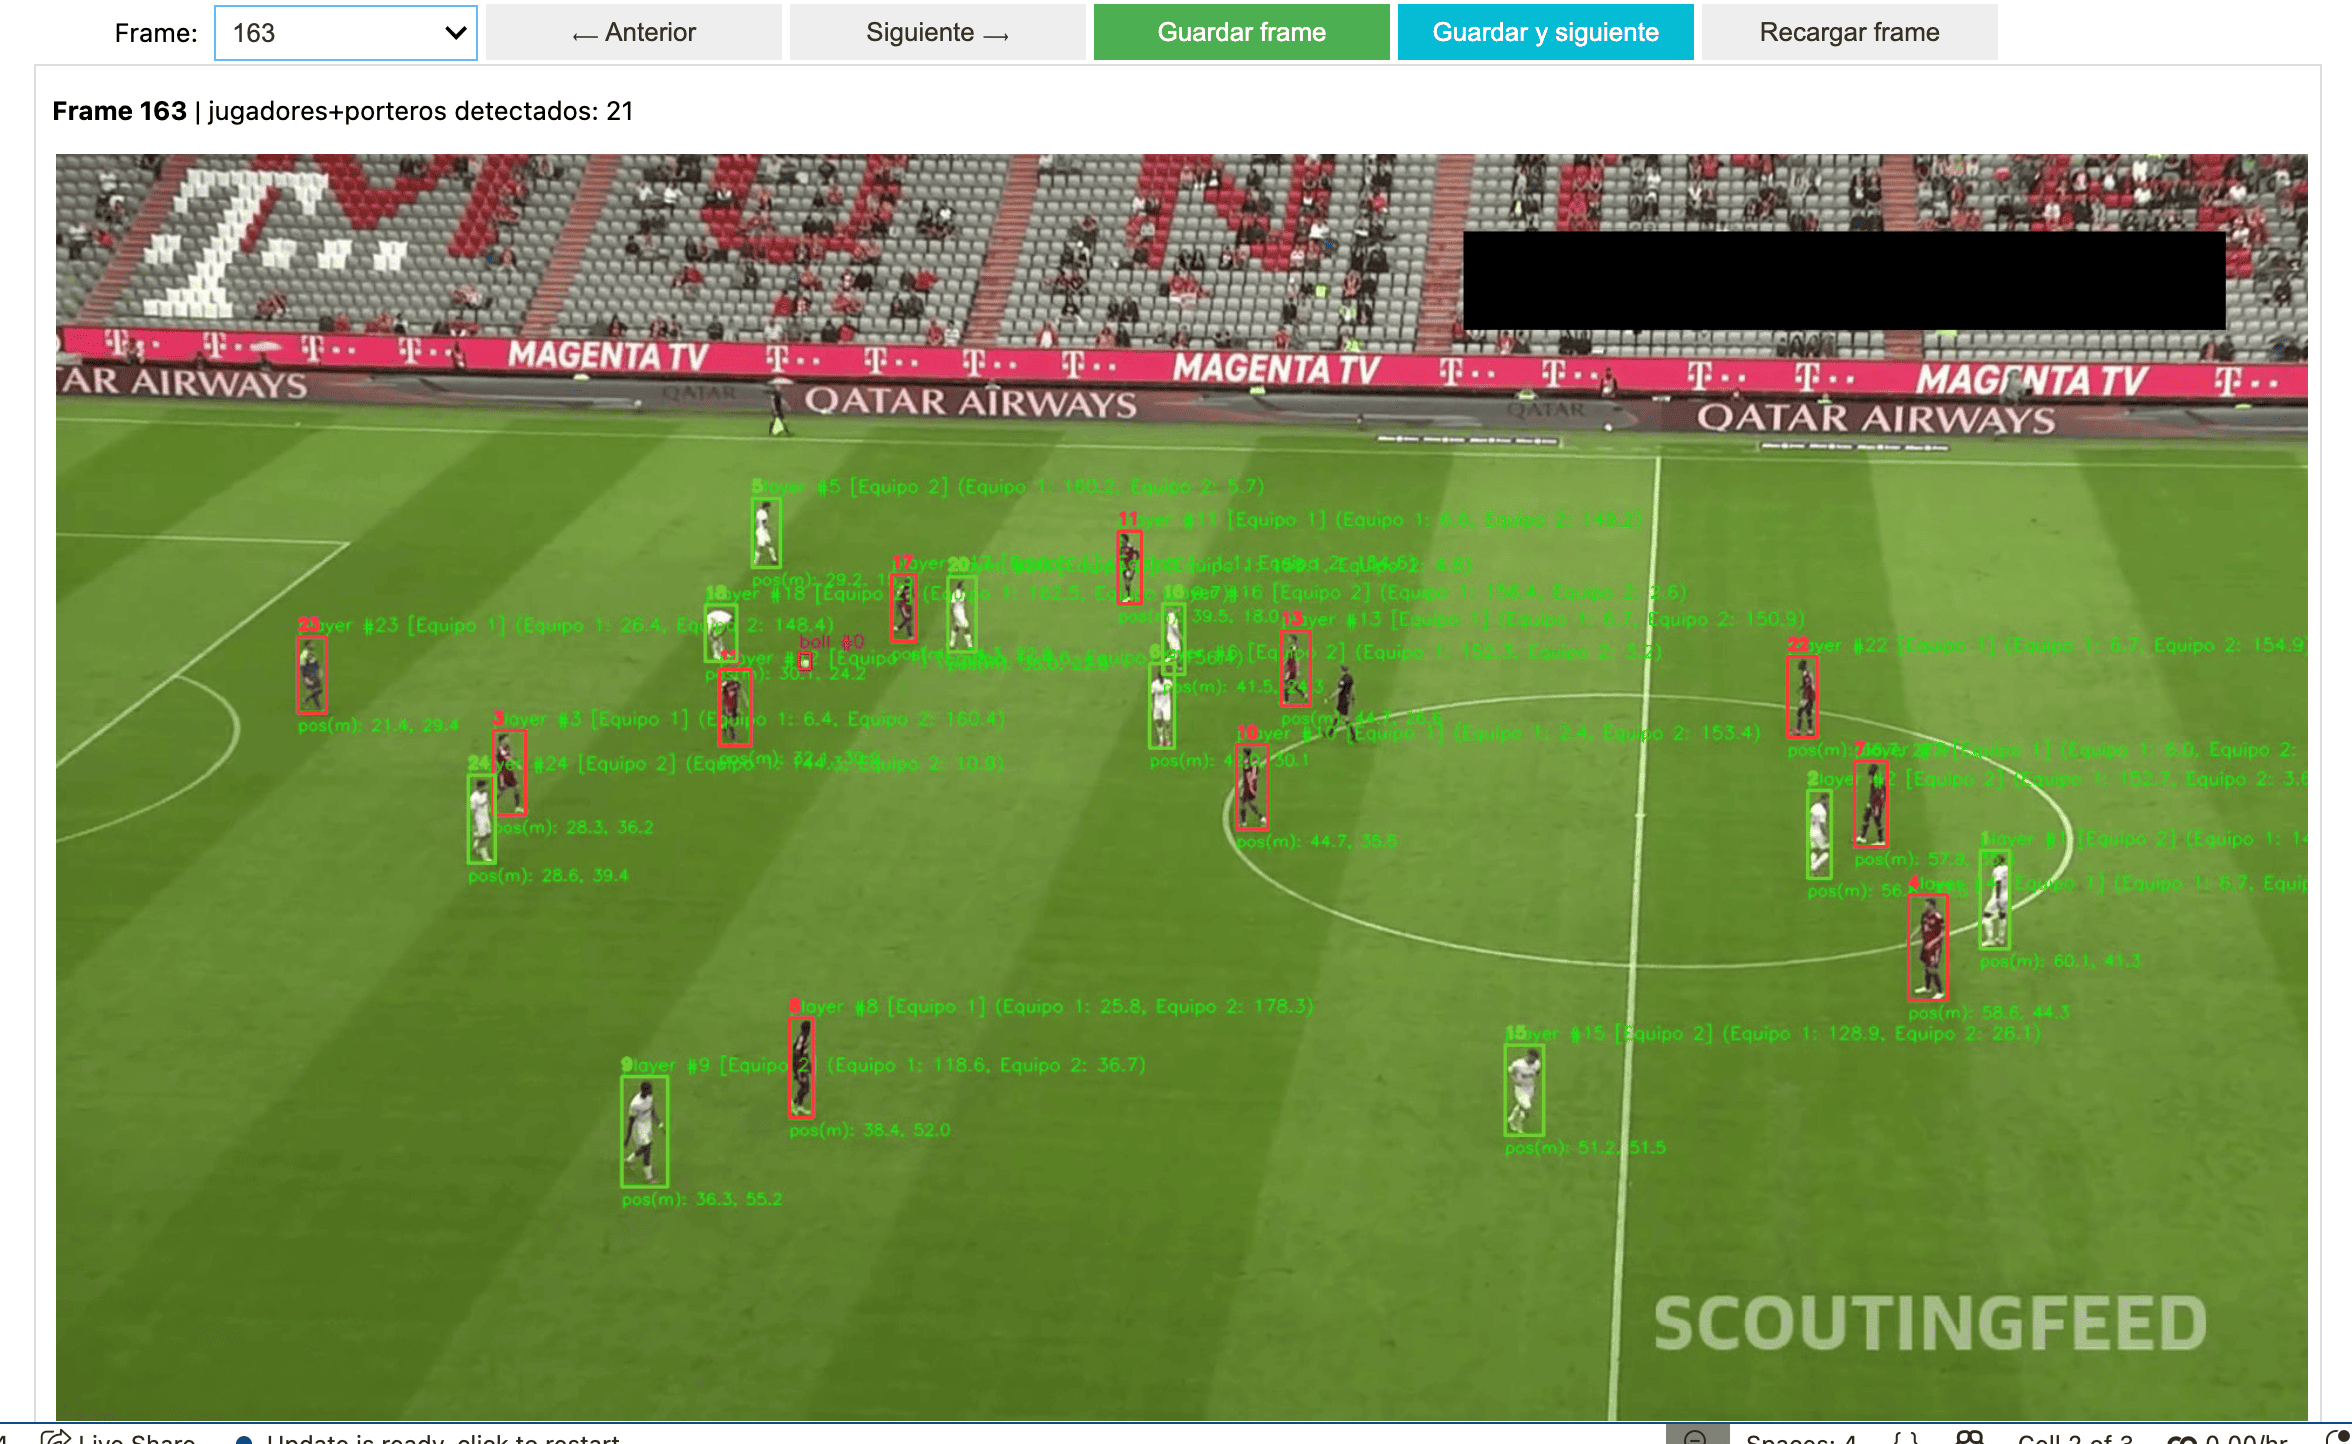
\includegraphics[width=0.49\linewidth]{Imagenes//Propias//Frame_a_etiquetar.png}
\caption{Frame con identificadores visibles sobre los jugadores para realizar el etiquetado posicional.}
\label{fig:frame_etiquetado_posiciones}
\end{figure}

\begin{figure}[H]
\centering
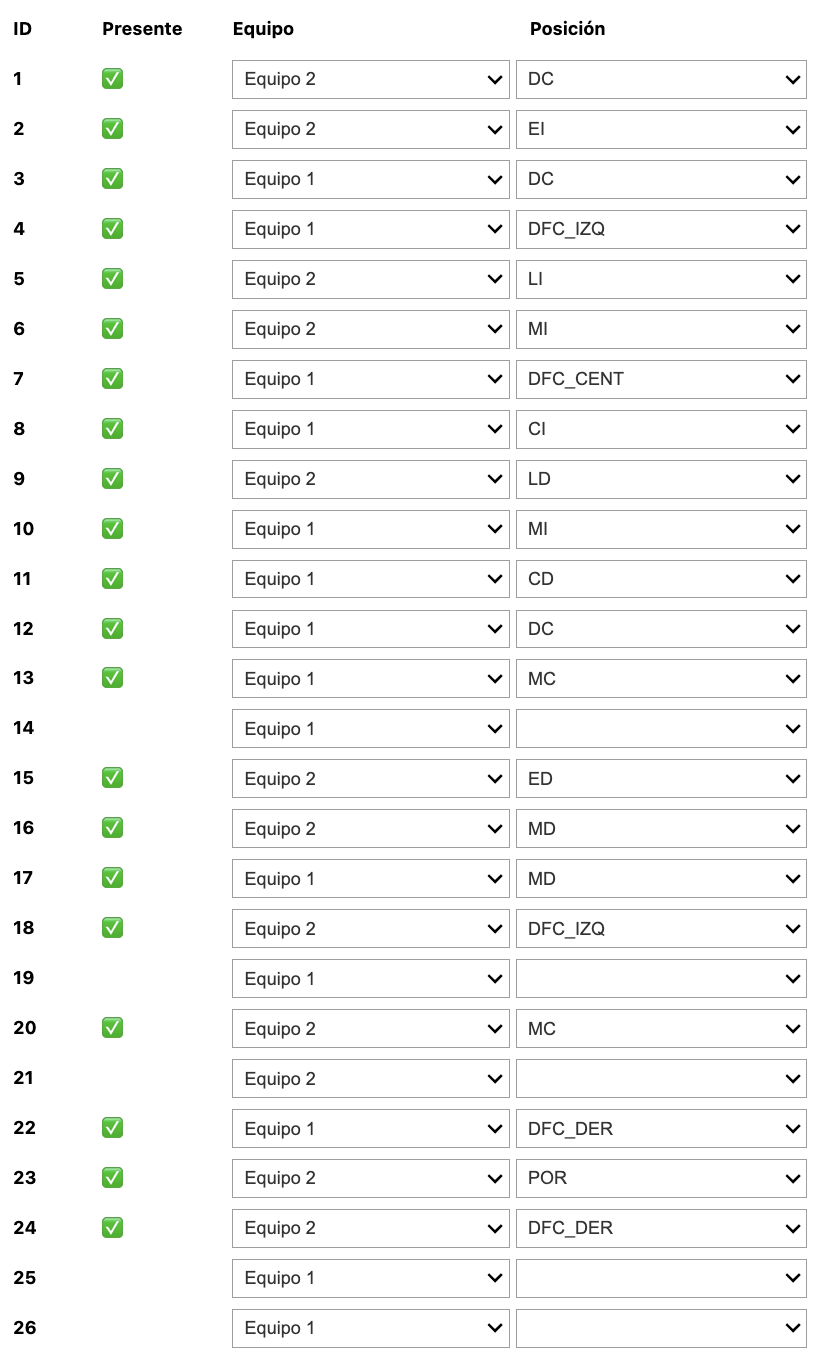
\includegraphics[width=0.49\linewidth]{Imagenes//Propias//Menu_para_etiquetar.png}
\caption{Menú de asignación de posición futbolística a cada identificador de tracking.}
\label{fig:menu_etiquetado_posiciones}
\end{figure}

\subsection{Variables utilizadas}

Cada muestra del dataset representa a un jugador objetivo en un frame concreto. Para describirlo se utilizan dos bloques de información: variables propias del jugador y variables relativas a sus compañeros.

Las variables del jugador objetivo son:

\begin{itemize}
    \item \texttt{x}, \texttt{y}: coordenadas normalizadas del jugador en el campo.
    \item \texttt{dist\_left\_sideline}: distancia normalizada a la banda izquierda.
    \item \texttt{dist\_right\_sideline}: distancia normalizada a la banda derecha.
    \item \texttt{dist\_own\_goal}: distancia normalizada a la portería propia.
    \item \texttt{dist\_opponent\_goal}: distancia normalizada a la portería rival.
    \item \texttt{team\_centroid\_x}, \texttt{team\_centroid\_y}: centroide del equipo en ese frame.
    \item \texttt{dx\_centroid}, \texttt{dy\_centroid}: desplazamiento del jugador respecto al centroide del equipo.
    \item \texttt{rank\_x\_team}, \texttt{rank\_y\_team}: posición relativa del jugador dentro del equipo según los ejes del campo.
    \item \texttt{vx}, \texttt{vy}: velocidad normalizada estimada a partir del desplazamiento entre frames.
\end{itemize}

Las variables de compañeros describen el contexto espacial del jugador objetivo. Para cada compañero se incluyen:

\begin{itemize}
    \item \texttt{dx\_to\_obj}, \texttt{dy\_to\_obj}: desplazamiento relativo respecto al jugador objetivo.
    \item \texttt{dist\_to\_obj}: distancia euclídea al jugador objetivo.
    \item \texttt{x}, \texttt{y}: posición normalizada del compañero.
    \item Distancias del compañero a bandas y porterías.
    \item \texttt{vx}, \texttt{vy}: velocidad normalizada del compañero.
\end{itemize}

Se consideran como máximo 10 compañeros por muestra, ordenados por cercanía al jugador objetivo. Cuando hay menos de 10 compañeros disponibles, se rellena con ceros y se utiliza una máscara para indicar qué posiciones son reales y cuáles son padding. En el dataset final, la mediana de compañeros visibles por muestra es 9.

\subsection{Normalización táctica del campo}

Un aspecto clave es que los equipos atacan en direcciones opuestas. Sin una normalización previa, un lateral izquierdo de un equipo podría aparecer en coordenadas similares a un lateral derecho del rival. Para evitarlo, todas las muestras se transforman a una misma vista táctica.

Si el equipo ataca hacia $+x$, las coordenadas se mantienen. Si ataca hacia $-x$, se aplica la transformación:

\[
x' = 1 - x
\]

\[
y' = 1 - y
\]

De esta manera, las etiquetas izquierda/derecha conservan el mismo significado para ambos equipos. Esta canonización es fundamental para que el modelo aprenda conceptos futbolísticos y no solo coordenadas absolutas dependientes del lado del campo.

\subsection{Distribución de clases}

El dataset inicial presentaba un desbalanceo claro. Las clases \texttt{CI}, \texttt{CD} y \texttt{DFC\_CENT} eran las menos representadas. Tras fusionar los carrileros con los laterales, el reparto quedó más equilibrado, aunque \texttt{DFC\_CENT} siguió siendo la clase minoritaria.

\begin{table}[H]
\centering
\scriptsize
\begin{tabular}{c|c|c}
\textbf{Clase} & \textbf{Muestras antes del mapeo} & \textbf{Muestras finales} \\
\hline\hline
\texttt{CI} & 2816 & -- \\
\hline
\texttt{CD} & 2094 & -- \\
\hline
\texttt{LI} & 8013 & 10829 \\
\hline
\texttt{LD} & 7681 & 9775 \\
\hline
\texttt{DFC\_CENT} & 2897 & 2897 \\
\hline
\texttt{DFC\_IZQ} & 11896 & 11896 \\
\hline
\texttt{DFC\_DER} & 11345 & 11345 \\
\hline
\texttt{MC} & 10946 & 10946 \\
\hline
\texttt{MI} & 10562 & 10562 \\
\hline
\texttt{MD} & 11480 & 11480 \\
\hline
\texttt{EI} & 8095 & 8095 \\
\hline
\texttt{ED} & 8029 & 8029 \\
\hline
\texttt{DC} & 13665 & 13665 \\
\hline
\end{tabular}
\caption{Distribución de clases antes y después de fusionar carrileros con laterales.}
\label{tab:position_class_distribution}
\end{table}

\subsection{Arquitectura del modelo}

El modelo utilizado es un Set Transformer. Esta arquitectura es adecuada porque el contexto de compañeros no es una secuencia ordenada, sino un conjunto. El orden en el que se introducen los compañeros no debería modificar la predicción. Si dos compañeros intercambian su posición en el tensor de entrada, la situación táctica sigue siendo la misma.

La entrada del modelo está formada por:

\begin{itemize}
    \item Un vector de 14 variables del jugador objetivo.
    \item Un tensor de compañeros de tamaño $10 \times 11$.
    \item Una máscara binaria que indica qué compañeros existen realmente y cuáles son padding.
\end{itemize}

El modelo se divide en cuatro etapas principales:

\begin{enumerate}
    \item Codificación del jugador objetivo.
    \item Codificación de cada compañero.
    \item Modelado del conjunto de compañeros mediante auto-atención.
    \item Agregación del conjunto y clasificación final.
\end{enumerate}

\subsubsection{Codificación del jugador objetivo}

El jugador objetivo se representa mediante sus 14 variables propias. Este vector se introduce en una MLP que lo transforma en un embedding de dimensión fija. Este embedding resume la información individual del jugador: dónde está, a qué distancia se encuentra de bandas y porterías, cómo se sitúa respecto al centroide de su equipo y qué posición relativa ocupa dentro del bloque.

Formalmente, si $x_{obj}$ es el vector de variables del jugador objetivo, se obtiene:

\[
h_{obj} = MLP_{obj}(x_{obj})
\]

donde $h_{obj}$ es el embedding individual del jugador.

\subsubsection{Codificación de los compañeros}

Cada compañero se representa mediante 11 variables. La misma MLP se aplica a todos los compañeros, de modo que todos se proyectan al mismo espacio latente:

\[
h_i = MLP_{comp}(x_i)
\]

donde $x_i$ representa las variables del compañero $i$ y $h_i$ su embedding. El resultado es un conjunto de embeddings:

\[
H = \{h_1, h_2, ..., h_n\}
\]

con $n \leq 10$. Si hay menos de 10 compañeros, los slots restantes se rellenan con ceros y se enmascaran.

\subsubsection{Bloques de auto-atención}

Sobre los embeddings de compañeros se aplican varios bloques de auto-atención multi-cabeza. En cada bloque, los compañeros actúan simultáneamente como consultas, claves y valores:

\[
Q = HW_Q,\quad K = HW_K,\quad V = HW_V
\]

La atención se calcula como:

\[
Attention(Q,K,V)=softmax\left(\frac{QK^T}{\sqrt{d_k}}\right)V
\]

Esta operación permite que el modelo aprenda relaciones entre compañeros. Por ejemplo, para distinguir entre un lateral y un extremo no basta con mirar la coordenada del jugador objetivo. También importa si existe un compañero por delante, si el jugador forma parte de una línea defensiva, si está alineado con otros mediocentros o si se encuentra aislado en zona de ataque.

La atención multi-cabeza permite aprender varias relaciones espaciales en paralelo. Una cabeza puede especializarse en relaciones longitudinales, otra en relaciones laterales, otra en distancias al centroide y otra en estructuras de línea defensiva o línea ofensiva.

Tras la atención se aplica una conexión residual y una normalización:

\[
Z_1 = LayerNorm(H + Attention(H))
\]

Después se aplica una red feed-forward interna:

\[
Z_2 = LayerNorm(Z_1 + FFN(Z_1))
\]

La red feed-forward contiene una expansión de dimensión, activación \texttt{GELU}, dropout y una proyección de vuelta a la dimensión original. Esta parte permite aprender transformaciones no lineales sobre las relaciones calculadas por la atención.

\subsubsection{Pooling por atención}

Después de los bloques de auto-atención, el modelo dispone de un embedding por cada compañero. Sin embargo, para clasificar al jugador objetivo se necesita un único vector que resuma el conjunto completo.

Para ello se utiliza pooling por atención mediante un vector aprendible llamado \textit{seed}. Este seed no representa a ningún jugador real. Funciona como una consulta global aprendida que pregunta qué información del conjunto de compañeros es relevante para clasificar al jugador objetivo.

En este bloque, el seed actúa como consulta $Q$, mientras que los compañeros actúan como claves $K$ y valores $V$:

\[
Q = S,\quad K = ZW_K,\quad V = ZW_V
\]

donde $S$ es el seed aprendible y $Z$ son los embeddings de compañeros tras los bloques de atención. El resultado es un único vector:

\[
h_{set} = PoolingAttention(S, Z)
\]

Este vector resume el contexto táctico del jugador objetivo.

\subsubsection{Clasificador final}

Finalmente, se concatena el embedding del jugador objetivo con el resumen del conjunto de compañeros:

\[
h = [h_{obj}; h_{set}]
\]

Este vector se introduce en un clasificador MLP que devuelve un logit por cada clase:

\[
logits = MLP_{cls}(h)
\]

Durante el entrenamiento se utiliza \texttt{CrossEntropyLoss}, que recibe directamente los logits. En inferencia, los logits se transforman en probabilidades mediante \texttt{softmax} y se selecciona la clase con mayor probabilidad.

\subsection{Entrenamiento}

La separación del dataset se realizó por partido, no por muestras individuales. Esto es importante porque los frames consecutivos de un mismo clip son muy parecidos. Si se mezclaran frames del mismo clip entre entrenamiento y test, las métricas estarían sobreestimadas.

El split final contiene:

\begin{itemize}
    \item 82122 muestras de entrenamiento.
    \item 13603 muestras de validación.
    \item 13794 muestras de test.
\end{itemize}

La función de pérdida utilizada fue \texttt{CrossEntropyLoss}. Para compensar el desbalanceo de clases se usaron pesos calculados a partir de la frecuencia de cada clase en entrenamiento. Además, en el modelo final se aplicó \texttt{label smoothing}, lo que suaviza las etiquetas y evita que el modelo se vuelva excesivamente confiado en clases que pueden ser tácticamente ambiguas.

La métrica principal para seleccionar el mejor modelo fue \textit{macro-F1}, ya que da el mismo peso a todas las clases.

\subsection{Grid search de hiperparámetros}

Para optimizar el modelo se realizaron varios barridos de hiperparámetros. Cada prueba se evaluó con métricas agregadas y con su matriz de confusión en test.

\subsubsection{Prueba 1: grid search con 13 clases}

La primera búsqueda mantuvo la taxonomía inicial, con \texttt{CI} y \texttt{CD} como clases independientes. Se ejecutaron 480 combinaciones variando anchura del modelo, regularización, número de bloques de atención, profundidad del codificador del jugador objetivo, expansión del feed-forward y tasa de aprendizaje.

La mejor configuración alcanzó un \textit{macro-F1} de 0.3096 en validación y 0.4022 en test.

\begin{table}[H]
\centering
\scriptsize
\begin{tabular}{c|c|c|c}
\textbf{Conjunto} & \textbf{Accuracy} & \textbf{Macro-F1} & \textbf{Weighted-F1} \\
\hline\hline
Validación & 0.3779 & 0.3096 & 0.3684 \\
\hline
Test & 0.4223 & 0.4022 & 0.4158 \\
\hline
\end{tabular}
\caption{Métricas de la mejor configuración del grid search con 13 clases.}
\label{tab:grid_13_metrics}
\end{table}

\begin{figure}[H]
\centering
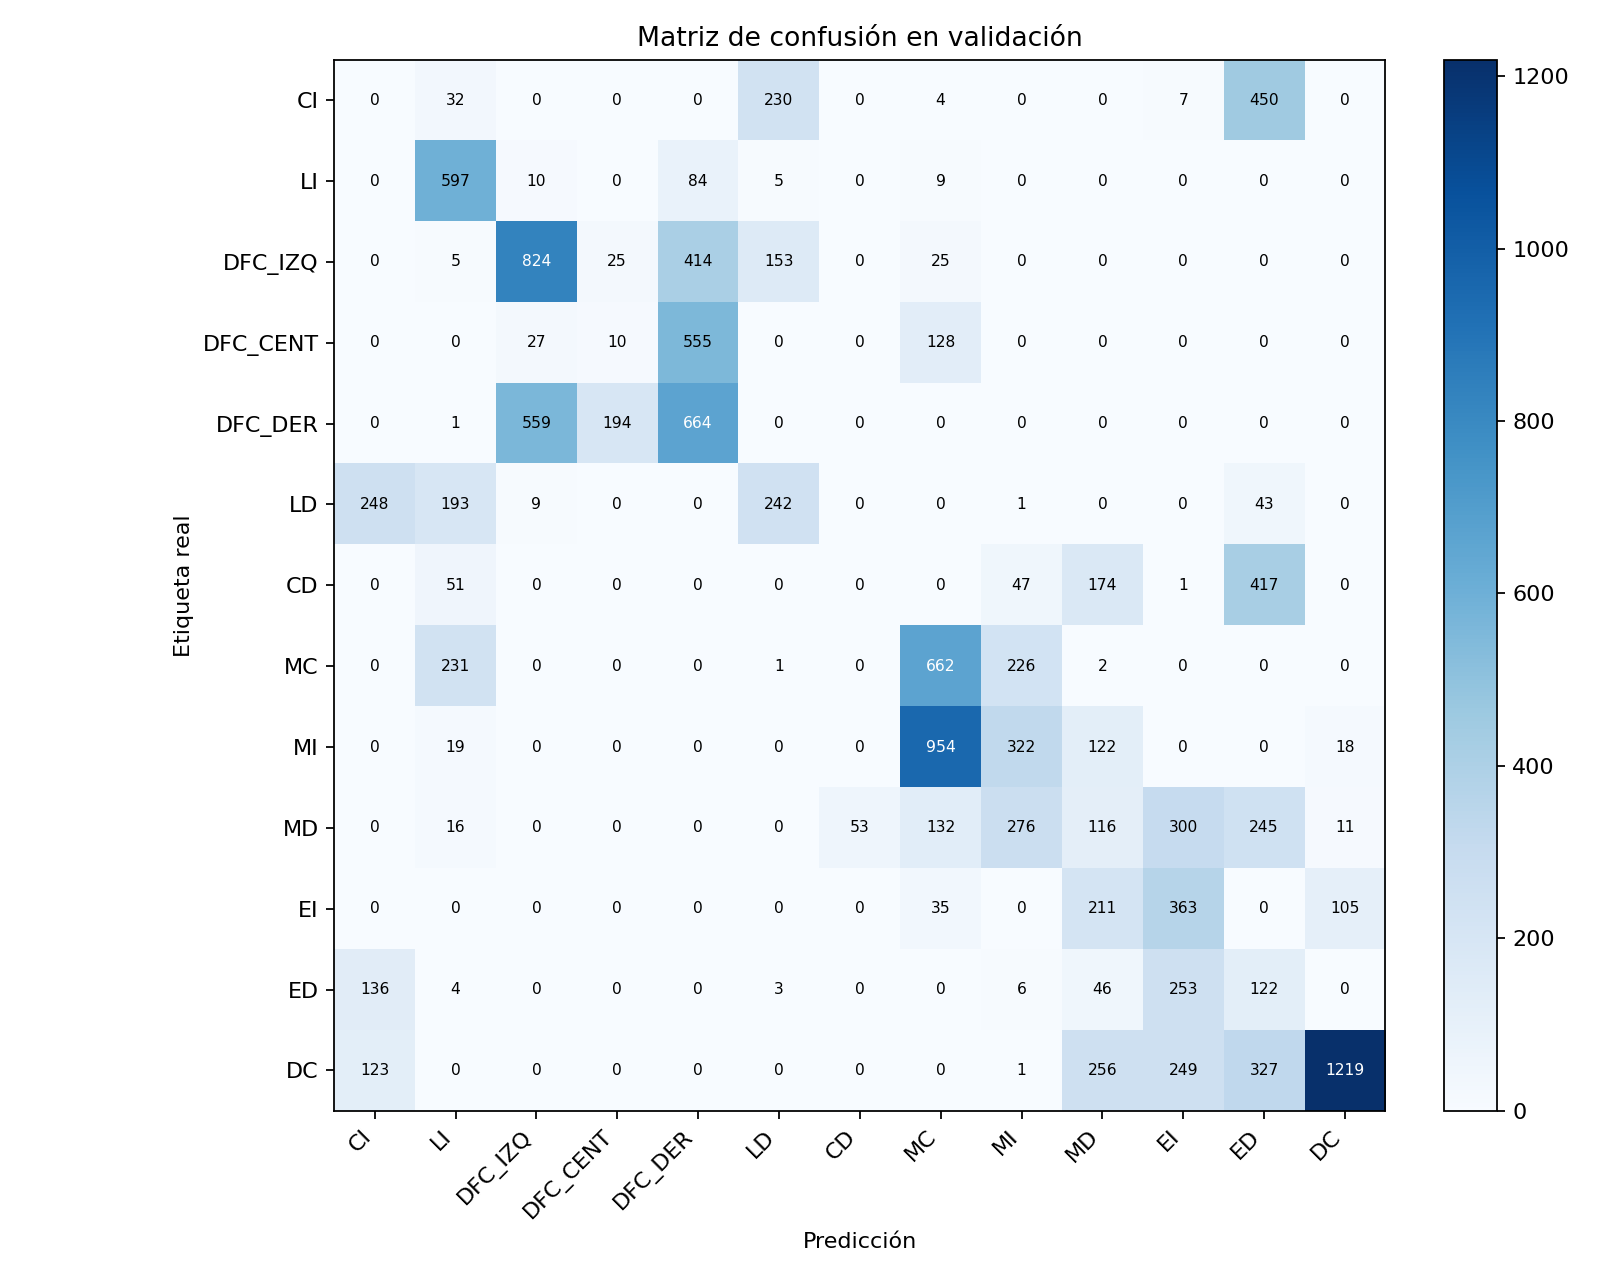
\includegraphics[width=0.49\linewidth]{Imagenes//Propias//matriz_confusion_grid_13.png}
\caption{Matriz de confusión en test del mejor modelo entrenado con 13 clases.}
\label{fig:confusion_grid_13}
\end{figure}

La matriz muestra que \texttt{CI} y \texttt{CD} eran clases inestables. En muchos casos se confundían con laterales, extremos o interiores. Esta observación motivó la fusión de carrileros con laterales.

\subsubsection{Prueba 2: fusión de carrileros con laterales}

En la segunda prueba se mantuvo la arquitectura anterior, pero se aplicó el mapeo:

\[
\texttt{CI} \rightarrow \texttt{LI},\quad \texttt{CD} \rightarrow \texttt{LD}
\]

El número de clases pasó de 13 a 11. El rendimiento aumentó de forma clara, especialmente en validación.

\begin{table}[H]
\centering
\scriptsize
\begin{tabular}{c|c|c|c}
\textbf{Conjunto} & \textbf{Accuracy} & \textbf{Macro-F1} & \textbf{Weighted-F1} \\
\hline\hline
Validación & 0.5563 & 0.5265 & 0.5628 \\
\hline
Test & 0.5240 & 0.4845 & 0.5156 \\
\hline
\end{tabular}
\caption{Métricas tras fusionar carrileros con laterales.}
\label{tab:grid_merged_metrics}
\end{table}

\begin{figure}[H]
\centering
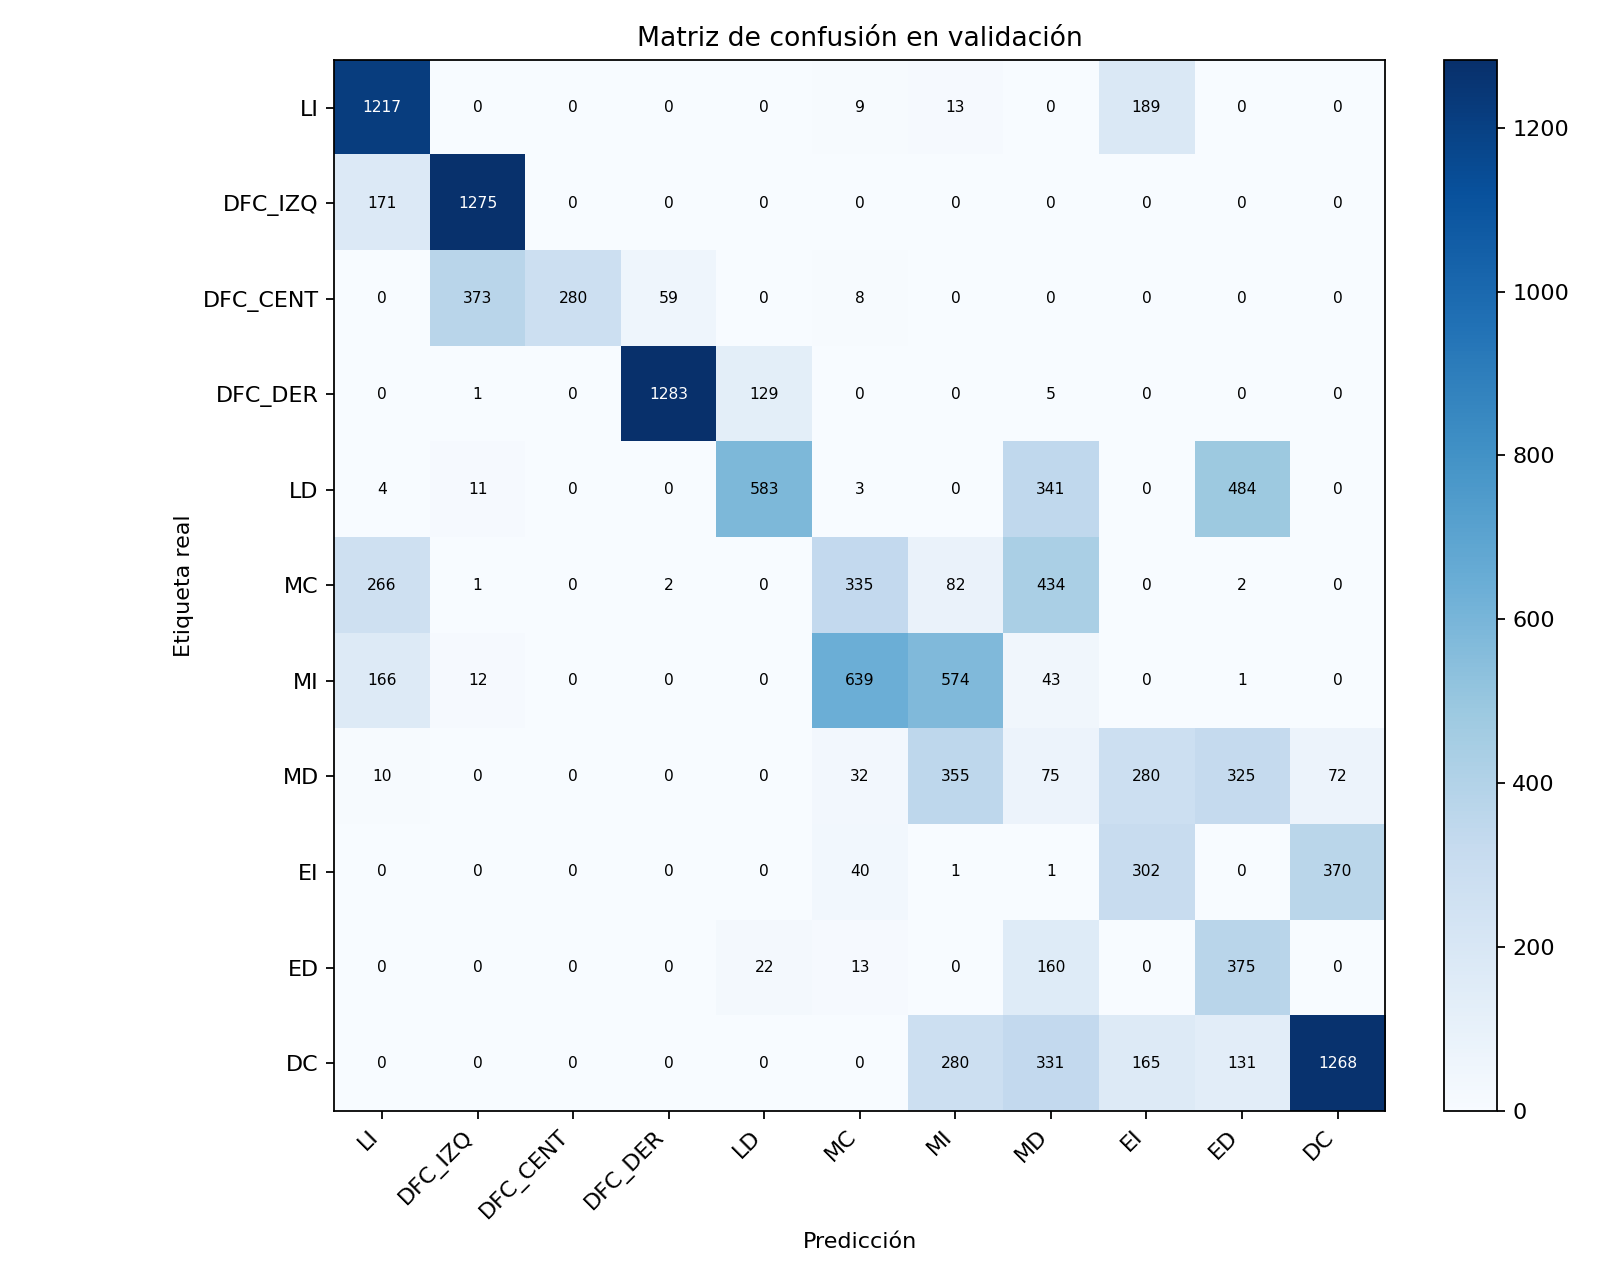
\includegraphics[width=0.49\linewidth]{Imagenes//Propias//matriz_confusion_carrileros_fusionados.png}
\caption{Matriz de confusión en test tras fusionar \texttt{CI} con \texttt{LI} y \texttt{CD} con \texttt{LD}.}
\label{fig:confusion_merged}
\end{figure}

Esta prueba confirmó que, con el volumen de datos disponible, separar carrileros y laterales introducía más ruido que información útil.

\subsubsection{Prueba 3: grid search completo con 11 clases}

Tras comprobar que el mapeo era beneficioso, se repitió un grid search completo con 11 clases. Se exploraron de nuevo 480 combinaciones. La mejor configuración utilizó una arquitectura más compacta, 5 bloques de atención y mayor regularización.

\begin{table}[H]
\centering
\scriptsize
\begin{tabular}{c|c|c|c}
\textbf{Conjunto} & \textbf{Accuracy} & \textbf{Macro-F1} & \textbf{Weighted-F1} \\
\hline\hline
Validación & 0.6168 & 0.5931 & 0.6207 \\
\hline
Test & 0.5170 & 0.4893 & 0.5096 \\
\hline
\end{tabular}
\caption{Métricas del grid search completo con 11 clases.}
\label{tab:grid_11_metrics}
\end{table}

\begin{figure}[H]
\centering
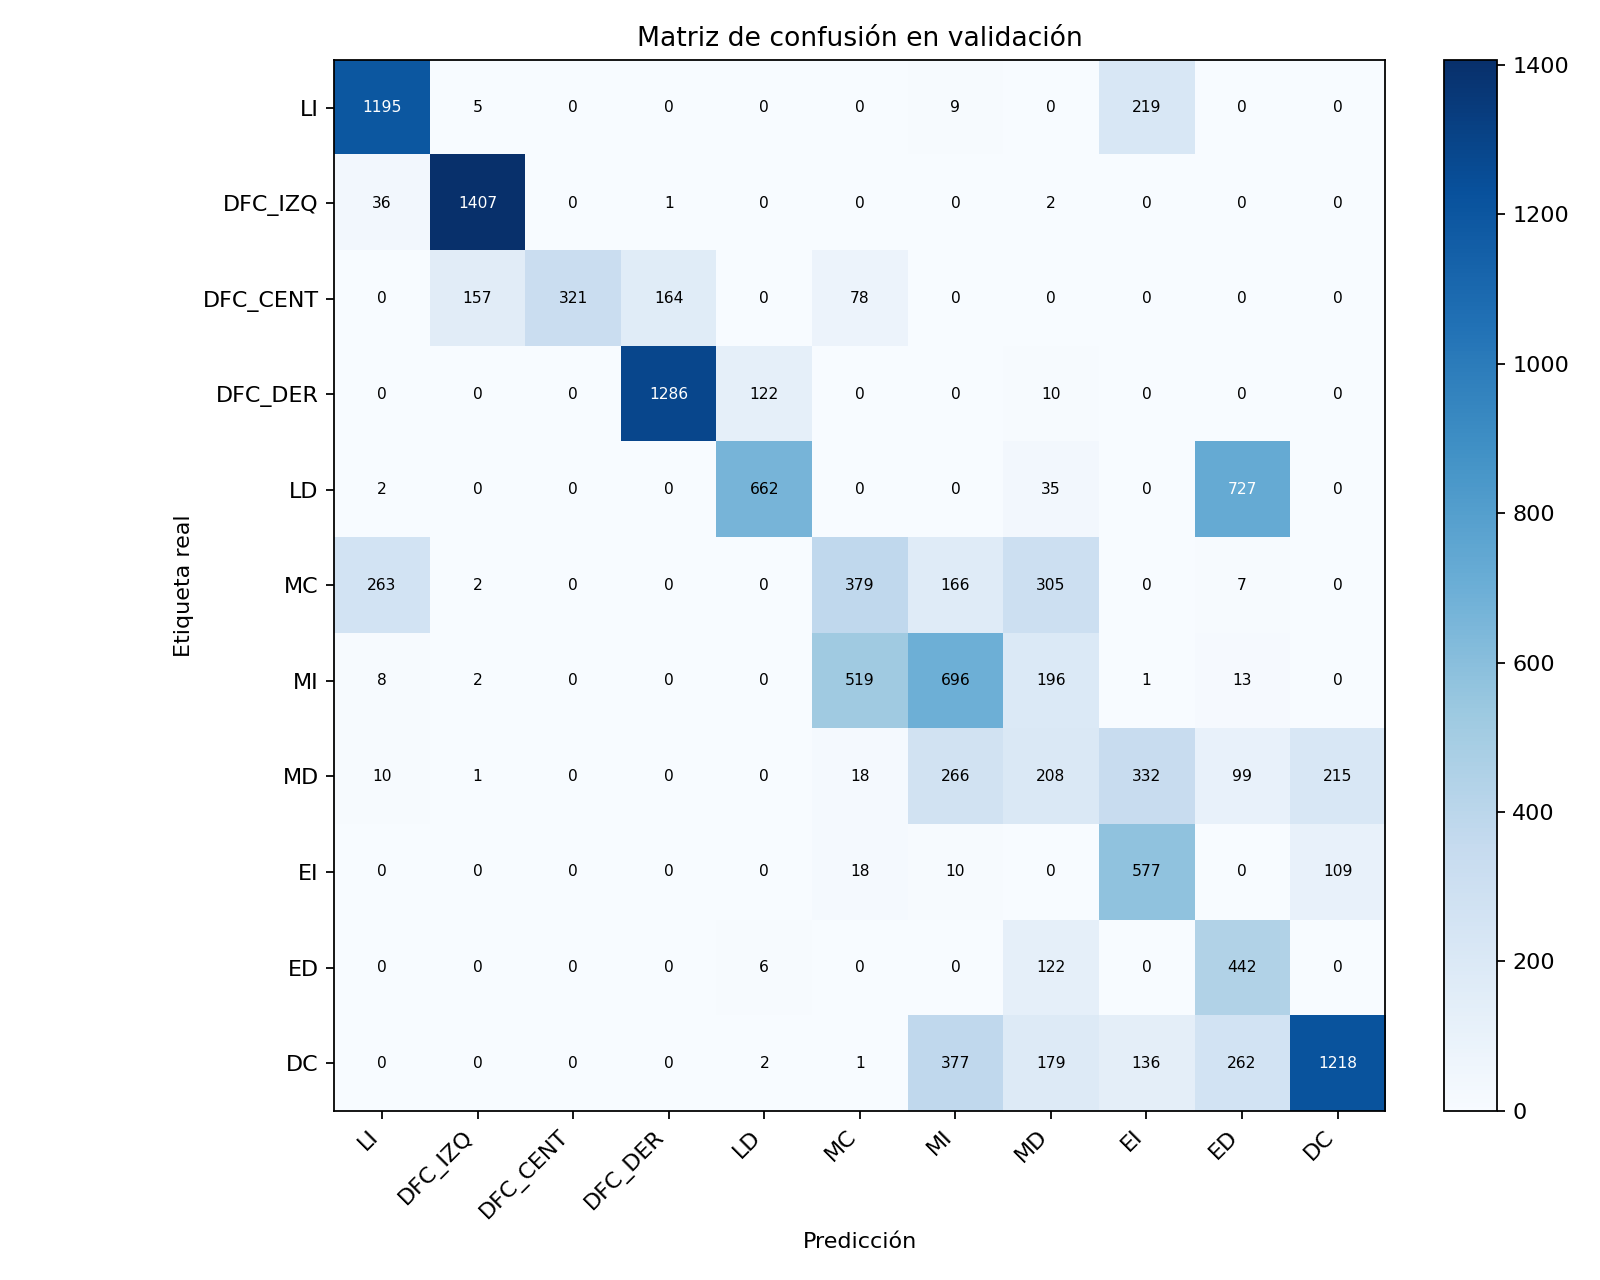
\includegraphics[width=0.49\linewidth]{Imagenes//Propias//matriz_confusion_grid_11.png}
\caption{Matriz de confusión en test del mejor modelo del grid search completo con 11 clases.}
\label{fig:confusion_grid_11}
\end{figure}

Aunque la validación mejoró claramente, el rendimiento en test no aumentó en la misma proporción. Esto sugiere que algunas configuraciones empezaban a adaptarse demasiado al clip de validación.

\subsubsection{Prueba 4: refinamiento de los tres mejores modelos}

En la última fase se tomaron los tres mejores modelos del grid anterior y se refinó alrededor de ellos. En lugar de volver a cruzar todos los parámetros, se mantuvieron fijas tres familias arquitectónicas y se probaron nuevos valores de \texttt{learning\_rate}, \texttt{weight\_decay}, \texttt{dropout} y \texttt{label\_smoothing}. En total se ejecutaron 108 entrenamientos.

El mejor modelo final obtuvo un \textit{macro-F1} de 0.6068 en validación y 0.5588 en test.

\begin{table}[H]
\centering
\scriptsize
\begin{tabular}{c|c|c|c}
\textbf{Conjunto} & \textbf{Accuracy} & \textbf{Macro-F1} & \textbf{Weighted-F1} \\
\hline\hline
Validación & 0.6333 & 0.6068 & 0.6358 \\
\hline
Test & 0.5804 & 0.5588 & 0.5703 \\
\hline
\end{tabular}
\caption{Métricas del modelo final tras el refinamiento de hiperparámetros.}
\label{tab:modelo_final_metricas}
\end{table}

\begin{figure}[H]
\centering
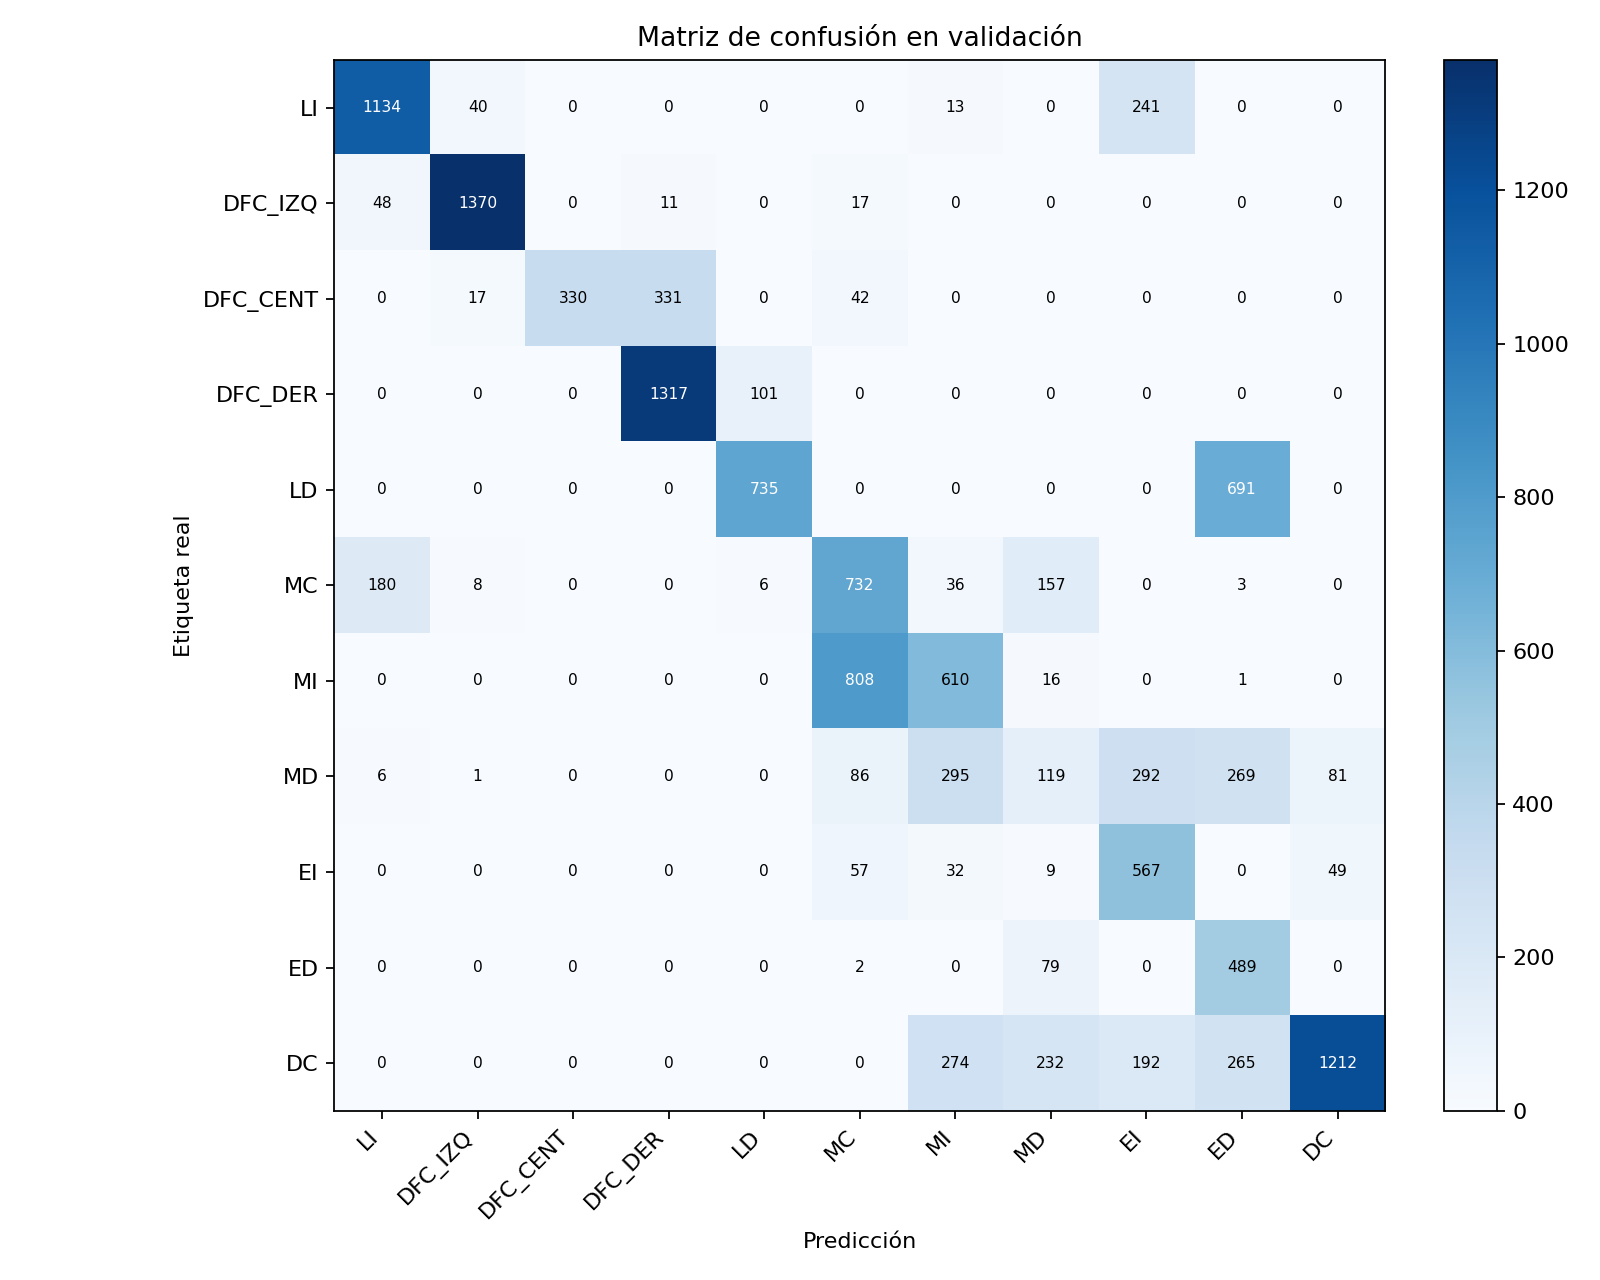
\includegraphics[width=0.49\linewidth]{Imagenes//Propias//matriz_confusion_modelo_final.png}
\caption{Matriz de confusión en test del modelo final.}
\label{fig:confusion_modelo_final}
\end{figure}

\begin{figure}[H]
\centering
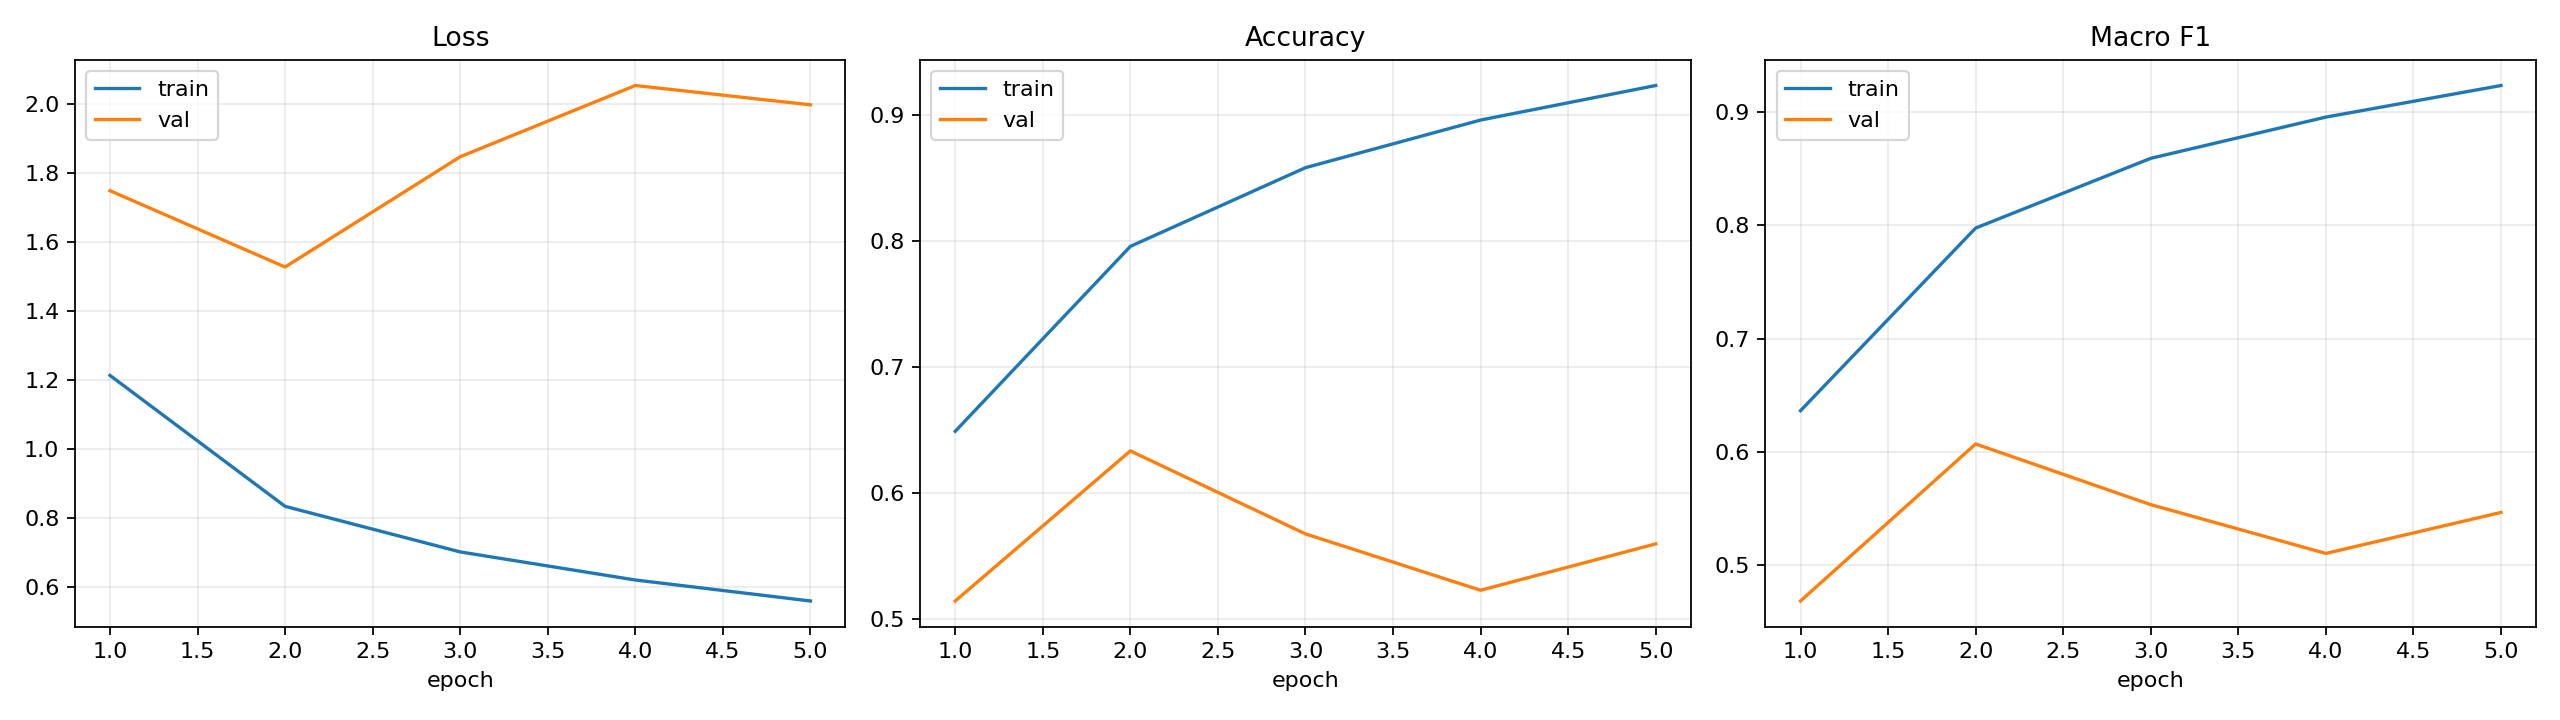
\includegraphics[width=0.49\linewidth]{Imagenes//Propias//curvas_entrenamiento_modelo_final.png}
\caption{Evolución de la pérdida, accuracy y macro-F1 durante el entrenamiento del modelo final.}
\label{fig:curvas_entrenamiento_modelo_final}
\end{figure}

La curva de entrenamiento muestra que el mejor punto se alcanza en las primeras épocas. A partir de ese momento, el rendimiento en entrenamiento sigue mejorando, pero la validación deja de mejorar de forma consistente. Este comportamiento indica sobreajuste temprano, algo esperable por la fuerte correlación entre frames de un mismo clip y por el tamaño limitado del conjunto de partidos etiquetados. Por ello se utiliza parada temprana y se selecciona el checkpoint con mayor \textit{macro-F1} de validación.

\subsection{Hiperparámetros del modelo final}

El modelo final utiliza la siguiente configuración:

\begin{table}[H]
\centering
\scriptsize
\begin{tabular}{c|c}
\textbf{Parámetro} & \textbf{Valor} \\
\hline\hline
\texttt{teammate\_embed\_dim} & 128 \\
\hline
\texttt{objective\_hidden\_dim} & 256 \\
\hline
\texttt{set\_hidden\_dim} & 256 \\
\hline
\texttt{fusion\_hidden\_dim} & 256 \\
\hline
\texttt{objective\_num\_layers} & 1 \\
\hline
\texttt{num\_set\_blocks} & 5 \\
\hline
\texttt{num\_heads} & 4 \\
\hline
\texttt{ff\_expansion} & 2 \\
\hline
\texttt{dropout} & 0.27 \\
\hline
\texttt{label\_smoothing} & 0.05 \\
\hline
\texttt{learning\_rate} & 0.0002 \\
\hline
\texttt{weight\_decay} & 0.0015 \\
\hline
\texttt{batch\_size} & 512 \\
\hline
\end{tabular}
\caption{Hiperparámetros del modelo final.}
\label{tab:hiperparametros_modelo_final}
\end{table}

El parámetro \texttt{teammate\_embed\_dim} controla la anchura de la MLP que codifica cada compañero antes de introducirlo en la atención. El parámetro \texttt{objective\_hidden\_dim} define la dimensión oculta usada para representar al jugador objetivo.

\texttt{set\_hidden\_dim} es la dimensión interna del Set Transformer. Es uno de los valores más importantes, ya que determina la capacidad del modelo para representar relaciones entre compañeros. \texttt{fusion\_hidden\_dim} define la anchura del clasificador final tras concatenar el embedding del jugador objetivo y el resumen del conjunto.

\texttt{objective\_num\_layers} indica cuántas capas ocultas tiene la MLP del jugador objetivo. En el modelo final se usa una única capa, lo que sugiere que las variables individuales son suficientemente expresivas y que añadir más profundidad aumentaba el riesgo de sobreajuste.

\texttt{num\_set\_blocks} indica cuántos bloques de auto-atención se aplican sobre los compañeros. El modelo final usa 5 bloques, permitiendo refinar varias veces las relaciones espaciales del conjunto. \texttt{num\_heads} indica el número de cabezas de atención en paralelo. Con 4 cabezas, el modelo puede aprender distintos tipos de relaciones tácticas simultáneamente.

\texttt{ff\_expansion} controla cuánto se expande la dimensión interna dentro del feed-forward de cada bloque de atención. \texttt{dropout} introduce regularización apagando aleatoriamente neuronas durante el entrenamiento. El valor final, 0.27, es relativamente alto, coherente con el sobreajuste observado.

\texttt{label\_smoothing} suaviza las etiquetas durante el entrenamiento. En vez de asignar probabilidad 1 a la clase correcta y 0 al resto, reparte una pequeña fracción de probabilidad entre las demás clases. Esto es útil porque algunas posiciones son tácticamente ambiguas.

\texttt{learning\_rate} controla el tamaño de los pasos del optimizador, y \texttt{weight\_decay} penaliza pesos demasiado grandes. Ambos contribuyen a estabilizar el entrenamiento y mejorar la generalización.

\subsection{Resultados por clase}

El modelo final alcanza una accuracy de 0.5804 y un \textit{macro-F1} de 0.5588 en test. Las mejores clases son \texttt{DFC\_IZQ}, \texttt{ED}, \texttt{DFC\_DER}, \texttt{DC} y \texttt{LI}. Las clases más difíciles son \texttt{DFC\_CENT}, \texttt{MD}, \texttt{MC} y \texttt{MI}.

\begin{table}[H]
\centering
\scriptsize
\begin{tabular}{c|c|c|c|c}
\textbf{Clase} & \textbf{Precisión test} & \textbf{Recall test} & \textbf{F1 test} & \textbf{Soporte test} \\
\hline\hline
\texttt{LI} & 0.6078 & 0.5985 & 0.6031 & 1432 \\
\hline
\texttt{DFC\_IZQ} & 0.9026 & 0.8560 & 0.8787 & 1451 \\
\hline
\texttt{DFC\_CENT} & 0.6272 & 0.1434 & 0.2335 & 739 \\
\hline
\texttt{DFC\_DER} & 0.5910 & 0.6723 & 0.6290 & 1367 \\
\hline
\texttt{LD} & 0.5820 & 0.5363 & 0.5582 & 1337 \\
\hline
\texttt{MC} & 0.4194 & 0.4783 & 0.4469 & 1403 \\
\hline
\texttt{MI} & 0.4724 & 0.4823 & 0.4773 & 1188 \\
\hline
\texttt{MD} & 0.4848 & 0.3457 & 0.4036 & 1478 \\
\hline
\texttt{EI} & 0.4263 & 0.9294 & 0.5845 & 694 \\
\hline
\texttt{ED} & 0.5464 & 0.9874 & 0.7035 & 715 \\
\hline
\texttt{DC} & 0.7674 & 0.5322 & 0.6285 & 1990 \\
\hline
\end{tabular}
\caption{Resultados por clase del modelo final sobre el conjunto de test.}
\label{tab:set_transformer_test_by_class}
\end{table}

Estos resultados son coherentes con la naturaleza de la tarea. Las posiciones de banda y algunos defensas tienen patrones espaciales más estables, mientras que los mediocentros e interiores dependen más de la fase de juego, de intercambios posicionales y del contexto colectivo.

\subsection{Reentrenamiento con \textit{train+val}}

Una vez seleccionado el mejor modelo mediante el \textit{grid search}, se realizó una prueba adicional para comprobar si el rendimiento podía mejorar utilizando más datos durante el entrenamiento. La idea consistía en unir los conjuntos de entrenamiento y validación, entrenar de nuevo el modelo con los hiperparámetros previamente seleccionados y evaluar el resultado únicamente sobre el conjunto de test. Esta prueba tiene sentido porque el modelo mostraba síntomas de sobreajuste temprano, por lo que cabía pensar que disponer de más muestras durante el entrenamiento podría mejorar su capacidad de generalización.

En esta prueba se entrenó el modelo durante 2 épocas, que era la época óptima obtenida en el proceso de validación anterior. El conjunto \textit{train+val} contenía 95725 muestras, mientras que el conjunto de test se mantuvo separado y no se utilizó para tomar decisiones durante el entrenamiento.

\begin{table}[H]
    \centering
    \begin{tabular}{c|c|c|c}
        \textbf{Modelo} & \textbf{Accuracy test} & \textbf{Macro-F1 test} & \textbf{Weighted-F1 test} \\
        \hline\hline
        Modelo seleccionado por validación & 0.5804 & 0.5588 & 0.5703 \\
        Reentrenado con \textit{train+val} & 0.5161 & 0.4833 & 0.5020 \\
        \hline
    \end{tabular}
    \caption{Comparación entre el modelo seleccionado en validación y el modelo reentrenado con \textit{train+val}.}
    \label{tab:comparacion_train_val_posiciones}
\end{table}

Como se observa en la Tabla \ref{tab:comparacion_train_val_posiciones}, el reentrenamiento con \textit{train+val} no mejoró los resultados en test. Aunque el modelo alcanzó sobre \textit{train+val} una \textit{accuracy} de 0.8890 y un \textit{macro-F1} de 0.8924, su rendimiento sobre test fue inferior al del modelo seleccionado mediante validación. Esto indica que añadir la partición de validación al entrenamiento no redujo el sobreajuste, sino que probablemente aumentó la adaptación del modelo a los fragmentos ya vistos. En este caso, todos los vídeos etiquetados proceden del mismo partido, por lo que la caída no se debe a un cambio completo de dominio entre partidos distintos. Por este motivo, se decidió mantener como modelo principal el seleccionado mediante validación, ya que ofrecía una mejor generalización sobre el fragmento reservado como test.


\subsection{Asignación táctica final de posiciones}

Tras obtener las probabilidades del Set Transformer, la inferencia no termina escogiendo simplemente la clase con mayor probabilidad para cada jugador. Esa predicción directa existe, pero se utiliza como una primera estimación libre. Posteriormente se aplica una fase de asignación táctica cuyo objetivo es que las posiciones finales sean coherentes con la alineación esperada de cada equipo.

Para cada jugador detectado, el modelo devuelve un vector de probabilidades sobre las clases aprendidas:

\[
p_i = 
\left[
p_i(\text{LI}),\,
p_i(\text{DFC\_IZQ}),\,
p_i(\text{DFC\_CENT}),\,
p_i(\text{DFC\_DER}),\,
p_i(\text{LD}),\,
p_i(\text{MC}),\,
p_i(\text{MI}),\,
p_i(\text{MD}),\,
p_i(\text{EI}),\,
p_i(\text{ED}),\,
p_i(\text{DC})
\right]
\]

La predicción libre de cada jugador se obtiene mediante la clase con mayor probabilidad:

\[
\hat{y}_i = \arg\max_c p_i(c)
\]

Sin embargo, esta predicción libre puede producir asignaciones tácticamente imposibles. Por ejemplo, varios jugadores podrían ser clasificados como delanteros, mientras que ninguna detección queda asignada a una posición defensiva concreta. Para corregir este problema se introduce el once esperado de cada equipo como una restricción posterior.

En primer lugar, las predicciones se agregan por jugador. En lugar de tomar una única predicción aislada de un frame, se promedian las probabilidades obtenidas a lo largo de las apariciones del mismo identificador:

\[
\bar{p}_i(c) = \frac{1}{T_i}\sum_{t=1}^{T_i} p_{i,t}(c)
\]

donde \(T_i\) representa el número de frames en los que el jugador \(i\) ha sido observado. Esta agregación reduce el ruido de las predicciones frame a frame y genera una estimación más estable de la posición real del jugador.

Los porteros se tratan como un caso especial. Como el modelo de posiciones se centra en jugadores de campo, si un track está identificado como portero, su posición se fija directamente como \texttt{POR} con confianza máxima. El resto de jugadores se asignan mediante una restricción global basada en el once esperado.

Antes de aplicar el algoritmo húngaro, se construye una matriz de costes entre jugadores y plazas tácticas. Esta fase previa es importante, porque el algoritmo húngaro no trabaja directamente sobre las etiquetas ganadoras del modelo, sino sobre un coste calculado para cada posible pareja jugador--posición.

Cada plaza esperada define un conjunto de etiquetas compatibles. En posiciones centrales la compatibilidad es estricta: una plaza \texttt{MC} se apoya en la probabilidad de \texttt{MC}, una plaza \texttt{DC} en la probabilidad de \texttt{DC}, y una plaza \texttt{DFC\_IZQ} en la probabilidad de \texttt{DFC\_IZQ}. En cambio, para las posiciones de banda se permite una compatibilidad por familia lateral. Una plaza izquierda puede apoyarse en \texttt{LI}, \texttt{MI} o \texttt{EI}; una plaza derecha puede apoyarse en \texttt{LD}, \texttt{MD} o \texttt{ED}. Esto permite corregir casos en los que el modelo detecta correctamente la banda del jugador, pero duda entre lateral, interior o extremo.

El coste entre el jugador \(i\) y la plaza esperada \(s\) se calcula escogiendo primero la mejor etiqueta compatible \(c\) para esa plaza:

\[
C_{i,s} =
\min_{c \in A_s}
\left(
-\log(\max(\bar{p}_i(c), \varepsilon))
+
P_{\text{comp}}(s,c)
+
P_{\text{geo}}(i,s)
\right)
\]

donde \(A_s\) es el conjunto de etiquetas compatibles con la plaza \(s\), \(\bar{p}_i(c)\) es la probabilidad media del jugador para la clase \(c\), \(P_{\text{comp}}\) es una penalización de compatibilidad entre etiqueta y plaza, y \(P_{\text{geo}}\) es una penalización geométrica.

La penalización geométrica compara la posición media del jugador con un punto de referencia táctico asociado a cada plaza. De esta forma, no solo se tiene en cuenta lo que predice el modelo, sino también si la zona media ocupada por el jugador encaja con la posición que se le intenta asignar. La distancia vertical se pondera ligeramente más que la horizontal para reflejar mejor la separación entre bandas:

\[
d((x_i,y_i), a_s) =
\sqrt{
(x_i - a_{s,x})^2
+
\left(1.20\,(y_i - a_{s,y})\right)^2
}
\]

y la penalización geométrica se obtiene aplicando un peso a esa distancia:

\[
P_{\text{geo}}(i,s) = 1.35 \cdot d((x_i,y_i), a_s)
\]

La penalización de compatibilidad vale cero cuando la etiqueta del modelo coincide exactamente con la plaza esperada. Si ambas pertenecen a la misma banda, pero no son exactamente iguales, se permite la asignación con una penalización adicional. En cambio, si una etiqueta de banda izquierda intenta apoyar una plaza derecha, o al revés, se introduce una penalización muy alta para evitar cruces incoherentes.

Una vez construida la matriz de costes, se aplica el algoritmo húngaro. Este algoritmo busca la asignación global de menor coste:

\[
\min_{\sigma}
\sum_i C_{i,\sigma(i)}
\]

Su función es garantizar que la solución final sea coherente a nivel de equipo, no solo jugador a jugador. En particular, evita que dos jugadores ocupen la misma plaza concreta del once esperado. Por tanto, la restricción correcta no es ``solo un jugador por posición'', sino ``solo un jugador por cada plaza esperada''. Si la formación contiene dos delanteros, existen dos plazas \texttt{DC}, por lo que dos jugadores pueden acabar asignados como delanteros.

El resultado final conserva varias informaciones: la posición libre predicha por el modelo, la posición restringida por el once esperado, la etiqueta del modelo que ha sustentado esa asignación y el coste de la asignación. Esto permite saber si una posición final procede de una coincidencia directa del modelo o de una corrección táctica posterior.

En caso de que existan más tracks de jugadores que plazas esperadas, los jugadores sobrantes no se incluyen en la asignación óptima principal. Para ellos se aplica una asignación de respaldo, escogiendo la mejor plaza compatible según el mismo criterio de probabilidad, compatibilidad y geometría. Esta asignación evita dejar jugadores sin posición, aunque no debe interpretarse como parte estricta del once táctico principal.

Durante el tracking online se añade además una fase de estabilización temporal. En lugar de congelar una posición a partir de una única predicción, se acumulan evidencias durante una ventana de frames: conteos de posiciones predichas, sumas de confianza, probabilidades medias y posición media en el campo. La estrategia utilizada prioriza las posiciones que dominan de forma consistente en el tiempo y, cuando quedan plazas por resolver, completa las asignaciones restantes mediante una optimización sobre los candidatos pendientes. Así se reduce el efecto de predicciones puntuales erróneas o de cambios momentáneos de zona durante el partido.

Finalmente, en formaciones con posiciones duplicadas, como el 4-4-2, se realiza una desambiguación adicional. En esta formación aparecen realmente dos mediocentros y dos delanteros. Para el modelo ambos se representan como \texttt{MC}, \texttt{MC} y \texttt{DC}, \texttt{DC}, ya que la red no predice explícitamente \texttt{MC\_IZQ}, \texttt{MC\_DCHO}, \texttt{DC\_IZQ} o \texttt{DC\_DCHO}. Una vez asignadas las plazas base, se comparan las distancias medias de esos jugadores a las bandas. El jugador más cercano a la banda izquierda se marca como \texttt{MC\_IZQ} o \texttt{DC\_IZQ}, mientras que el más cercano a la banda derecha se marca como \texttt{MC\_DCHO} o \texttt{DC\_DCHO}. Esta separación permite asociar correctamente cada track con el nombre del jugador introducido en la alineación.
